\documentclass[conference]{IEEEtran}
\usepackage{cite}
\usepackage{amsmath,amssymb,amsfonts}
\usepackage{graphicx}
\usepackage{booktabs}
\usepackage{url}
\usepackage{xcolor}

\begin{document}

\title{Self-Supervised 2D+3D Hybrid GraphGPS for Multi-Objective ADMET Profiling, Explainable Safety Scoring, and Evolutionary Lead Optimization}

\author{\IEEEauthorblockN{Prathmesh Toke}
\IEEEauthorblockA{Department of Computer Science and Engineering\\
Computational Drug Discovery \& Graph Representation Learning\\
Email: tokeprathmesh54321@gmail.com}}

\maketitle

\begin{abstract}
Pre-clinical drug discovery exhibits over a 90\% attrition rate, predominantly driven by poor absorption, distribution, metabolism, excretion, and toxicity (ADMET) profiles such as fatal hERG cardiotoxicity and low oral bioavailability. Training supervised graph neural networks (GNNs) on clinical assays is severely constrained by sparse, imbalanced, and incomplete endpoint tables, while standard message-passing GNNs suffer from 1-hop local myopia, oversmoothing, and insensitivity to three-dimensional (3D) conformation. Furthermore, naive random dataset splits leak near-identical chemical scaffolds across training and test sets, yielding inflated generalization estimates. To address these bottlenecks, we introduce an end-to-end Self-Supervised 2D+3D Hybrid GraphGPS framework evaluated on 10,007 standardized compounds: 5,000 unlabeled ZINC250k molecules for leakage-free contrastive pre-training and 5,007 unique clinical compounds across 3,137 Bemis-Murcko scaffolds curated from Therapeutics Data Commons (TDC). Each molecular graph combines 29-dimensional chemical and 3D conformer atom features, 8-dimensional bond descriptors, sign-canonicalized Laplacian positional encodings (LapPE), sign-invariant random-walk structural encodings (RWSE), and ETKDGv3 global 3D shape vectors. A parallel local covalent TransformerConv and global all-atom MultiheadAttention backbone is pre-trained via undirected-symmetric GraphCL InfoNCE loss (converging from 0.8659 to 0.0402) and fine-tuned via NaN-masked, class-weighted multi-task heads. On a strictly unseen-scaffold held-out test set (n = 502), our SSL-GraphGPS achieves 0.8299 Macro ROC-AUC across Oral Bioavailability (0.7769), BBB Permeability (0.9001), and hERG Cardiotoxicity (0.8128), plus R\textsuperscript{2} = 0.7165 on QED and R\textsuperscript{2} = 0.7584 on SAScore---outperforming Random Forest ECFP4 (0.8070), Standard-GCN (0.8066), and GraphGPS-Scratch (0.7956) on every endpoint. Finally, pairing 23 medicinal chemistry SMIRKS rules, BRICS fragment recombination, PAINS/Lipinski filters, NSGA-II Pareto sorting, and Input $\times$ Gradient atom saliency yields interpretable, synthesizable lead candidates.
\end{abstract}

\begin{IEEEkeywords}
ADMET prediction, GraphGPS, Graph Transformer, self-supervised learning, InfoNCE, Bemis-Murcko scaffold split, Pareto optimization, explainable AI, hERG cardiotoxicity.
\end{IEEEkeywords}

\section{Introduction}
Bringing a single new drug to market requires 10--15 years and over \$2.6 billion in capitalized research and development expenditure \cite{DiMasi2016}, yet more than 90\% of candidates fail during human clinical trials \cite{Waring2015}. Retrospective pharmaceutical analyses demonstrate that poor pharmacokinetics and safety liabilities---collectively termed ADMET (Absorption, Distribution, Metabolism, Excretion, and Toxicity)---account for a substantial fraction of late-stage attrition \cite{Waring2015}. Specifically, low oral bioavailability ($F < 20\%$) prevents therapeutic systemic exposure \cite{Ma2008Bioavailability}, unintended Blood-Brain Barrier (BBB) penetration triggers central nervous system (CNS) side effects for peripheral drugs \cite{Martins2012BBB}, and off-target inhibition of the cardiac hERG potassium channel induces fatal QT-interval prolongation \cite{Wang2016hERG,Karim2021CardioTox}.

Despite the urgency of computational ADMET screening, deep learning approaches face four coupled challenges:
\begin{enumerate}
    \item \emph{Clinical Data Scarcity and Missing Assays:} Public clinical ADMET tables rarely cover more than several hundred to a few thousand molecules \cite{Huang2021TDC}, and experimental endpoints are sparsely observed across compound libraries (resulting in large numbers of missing \texttt{NaN} entries when combining assays).
    \item \emph{Architectural Myopia and 2D Blindness:} Standard Graph Convolutional Networks (GCNs) \cite{Kipf2017GCN} propagate messages strictly across 1-hop covalent bonds, suffer oversmoothing when stacked deeply, and omit bond attributes and 3D spatial conformation \cite{Riniker2015ETKDG,Rampasek2022GraphGPS}.
    \item \emph{Structural Data Leakage:} Conventional random splitting places structural analogues sharing identical core rings into both training and test folds, inflating evaluation metrics relative to true out-of-distribution scaffold generalization \cite{Bemis1996Murcko}.
    \item \emph{Single-Objective Lead Design Flaws:} Optimizing potency or absorption alone frequently degrades cardiac safety or synthetic feasibility, requiring explicit multi-objective trade-off resolution \cite{Derringer1980Desirability,Deb2002NSGA2} and chemically interpretable attribution \cite{Shrikumar2017InputGrad}.
\end{enumerate}

To resolve all four gaps in a reproducible framework, we make the following concrete contributions:
\begin{itemize}
    \item \textbf{Leakage-Free Real-World Multi-Task Benchmark:} We standardize and merge four Therapeutics Data Commons (TDC) clinical datasets \cite{Huang2021TDC,Ma2008Bioavailability,Martins2012BBB,Wang2016hERG,Karim2021CardioTox} with exact RDKit QED \cite{Bickerton2012QED} and SAScore \cite{Ertl2009SAScore} descriptors into 5,007 compounds across 3,137 Bemis-Murcko scaffolds \cite{Bemis1996Murcko}, alongside 5,000 ZINC250k unlabeled molecules \cite{GomezBombarelli2018,Sterling2015ZINC} filtered for zero scaffold/SMILES overlap with validation and test sets.
    \item \textbf{2D+3D Hybrid Local+Global GraphGPS Architecture:} Extending the GraphGPS recipe \cite{Rampasek2022GraphGPS} and edge-aware attention \cite{Shi2021TransformerConv}, our encoder combines local bond-aware \texttt{TransformerConv} with dense all-atom \texttt{MultiheadAttention}, sign-canonicalized Laplacian PE + RWSE \cite{Dwivedi2022LSPE}, and fast ETKDGv3 3D conformer geometry \cite{Riniker2015ETKDG}.
    \item \textbf{Undirected-Safe GraphCL Pre-Training \& Masked Multi-Task Learning:} We design undirected-symmetric edge dropping and subgraph node dropping \cite{You2020GraphCL,Wang2022MolCLR} for InfoNCE pre-training \cite{Chen2020SimCLR}, coupled with \texttt{NaN}-masked class-weighted logits and normalized regression losses.
    \item \textbf{Evolutionary Pareto Lead Optimization \& Atom Saliency XAI:} We combine 23 medicinal chemistry SMIRKS transformations, BRICS fragment recombination \cite{Degen2008BRICS}, PAINS/Lipinski filtering \cite{Baell2010PAINS,Lipinski2001Ro5}, Derringer-Suich desirability \cite{Derringer1980Desirability}, NSGA-II Pareto peeling \cite{Deb2002NSGA2}, and Input $\times$ Gradient attribution \cite{Shrikumar2017InputGrad}.
\end{itemize}

\section{Related Work}
\subsection{Classical Chemoinformatics and QSAR Modeling}
Quantitative Structure-Activity Relationship (QSAR) baselines historically rely on fixed circular bit-vector encodings such as Extended-Connectivity Fingerprints (ECFP4) \cite{Rogers2010ECFP} paired with tree ensembles like Random Forests \cite{Breiman2001RF}. While computationally fast and strong at memorizing local functional groups, ECFP4 bit-vectors suffer hash collisions, omit long-range inter-atomic spatial relationships, discard 3D molecular shape, and train independent single-task models unable to share pharmacological representations across endpoints.

\subsection{Message-Passing GNNs and Graph Transformers}
Kipf and Welling \cite{Kipf2017GCN} popularized spectral-inspired Graph Convolutional Networks (GCNs) operating on graph adjacency matrices. However, pure 1-hop message passing fails to capture non-bonded intramolecular electrostatic interactions and exhibits oversmoothing across deeper stacks. Shi et al. \cite{Shi2021TransformerConv} introduced masked graph attention incorporating edge embeddings (\texttt{TransformerConv}), yet attention restricted solely to covalent edges remains locally bounded. Ramp{\'a}{\v{s}}ek et al. \cite{Rampasek2022GraphGPS} demonstrated in GraphGPS that fusing parallel local message passing with global full-graph self-attention and structural/positional encodings (LSPE/RWSE \cite{Dwivedi2022LSPE}) achieves strong expressivity. We adapt GraphGPS specifically for drug discovery by integrating fast RDKit ETKDGv3 3D conformer descriptors \cite{Riniker2015ETKDG} and canonicalizing eigenvector sign ambiguity.

\subsection{Self-Supervised Molecular Pre-Training}
Inspired by SimCLR \cite{Chen2020SimCLR} in computer vision, GraphCL \cite{You2020GraphCL} and MolCLR \cite{Wang2022MolCLR} established contrastive learning over molecular graphs via InfoNCE loss. A subtle implementation pitfall in molecular contrastive learning is breaking graph symmetry when dropping directed edge indices independently or omitting desalting before positional encoding. Our implementation enforces canonical undirected bond symmetry during edge perturbation and evaluates transfer strictly on unseen scaffolds.

\subsection{Multi-Objective Lead Design and Explainability}
Automated molecular design frameworks \cite{GomezBombarelli2018} and fragment assembly toolkits such as BRICS \cite{Degen2008BRICS} generate candidate analogues around seed leads, which must obey Lipinski oral drug-likeness constraints \cite{Lipinski2001Ro5} and pass Pan-Assay Interference Compounds (PAINS) structural filters \cite{Baell2010PAINS}. Balancing conflicting ADMET goals mathematically leverages Derringer-Suich geometric desirability \cite{Derringer1980Desirability} and NSGA-II non-dominated sorting \cite{Deb2002NSGA2}, while Input $\times$ Gradient attribution \cite{Shrikumar2017InputGrad} verifies that neural predictions align with medicinal chemistry pharmacophores \cite{Wang2016hERG}.

\section{Dataset Curation and Zero-Leakage Protocol}
To evaluate generalization under realistic medicinal chemistry deployment, all compounds are processed through RDKit \texttt{LargestFragmentChooser} desalting, sanitization, heavy-atom bounds filtering ($[2, 80]$ heavy atoms with carbon presence), and canonical non-isomeric SMILES deduplication.

\subsection{Multi-Task Clinical ADMET and Unlabeled SSL Corpora}
Clinical binary endpoints are sourced from TDC \cite{Huang2021TDC}: \texttt{Bioavailability\_Ma} \cite{Ma2008Bioavailability} (human oral bioavailability $F \ge 20\%$), \texttt{BBB\_Martins} \cite{Martins2012BBB} (blood-brain barrier permeability), \texttt{hERG} \cite{Wang2016hERG} ($n=655$), and a stratified balanced subsample ($n=2{,}500$) from \texttt{hERG\_Karim} \cite{Karim2021CardioTox}. Duplicate canonical SMILES across sources are resolved via assay majority vote (dropping exact 50/50 conflicts). Continuous QED \cite{Bickerton2012QED} and SAScore \cite{Ertl2009SAScore} ground-truth targets are computed for all 5,007 unique merged molecules ($\text{QED}=0.595 \pm 0.197$, $\text{SAScore}=3.226 \pm 0.940$). For contrastive pre-training, 5,000 drug-like molecules are sampled from ZINC250k \cite{GomezBombarelli2018,Sterling2015ZINC} after explicitly removing any molecule sharing a canonical SMILES or Bemis-Murcko scaffold \cite{Bemis1996Murcko} with ADMET validation or test splits.

\subsection{Disjoint Bemis-Murcko Scaffold Splitting}
We partition the 5,007 ADMET molecules into 80\% training, 10\% validation, and 10\% test sets by grouping compounds on their Bemis-Murcko ring-and-linker scaffolds \cite{Bemis1996Murcko}, guaranteeing every validation and test compound resides on a completely unseen core structure (Table~\ref{tab:dataset} and Fig.~\ref{fig:eda}). Automated assertions verify zero scaffold overlap and zero SMILES overlap across all splits while ensuring both binary classes appear in every split.

\begin{table}[t]
\centering
\caption{Curated Multi-Task ADMET Dataset and Disjoint Bemis-Murcko Scaffold Split Summary}
\label{tab:dataset}
\setlength{\tabcolsep}{4pt}
\begin{tabular}{lcccc}
\toprule
\textbf{Split / Set} & \textbf{Mols (Scaffolds)} & \textbf{Bioavail. (+\%)} & \textbf{BBB (+\%)} & \textbf{hERG (+\%)} \\
\midrule
SSL Unlabeled & 5,000 (ZINC250k) & --- & --- & --- \\
Train (80\%)  & 4,005 (2,135) & 536 (78.0\%) & 1,611 (75.9\%) & 2,252 (54.2\%) \\
Val (10\%)    & 500 (500)     & 56 (67.9\%)  & 157 (80.3\%)   & 317 (55.5\%) \\
Test (10\%)   & 502 (502)     & 44 (75.0\%)  & 153 (82.4\%)   & 330 (48.5\%) \\
\midrule
\textbf{Total ADMET} & \textbf{5,007 (3,137)} & \textbf{636 (76.9\%)} & \textbf{1,921 (76.7\%)} & \textbf{2,899 (53.7\%)} \\
\bottomrule
\end{tabular}
\end{table}

\begin{figure}[t]
\centering
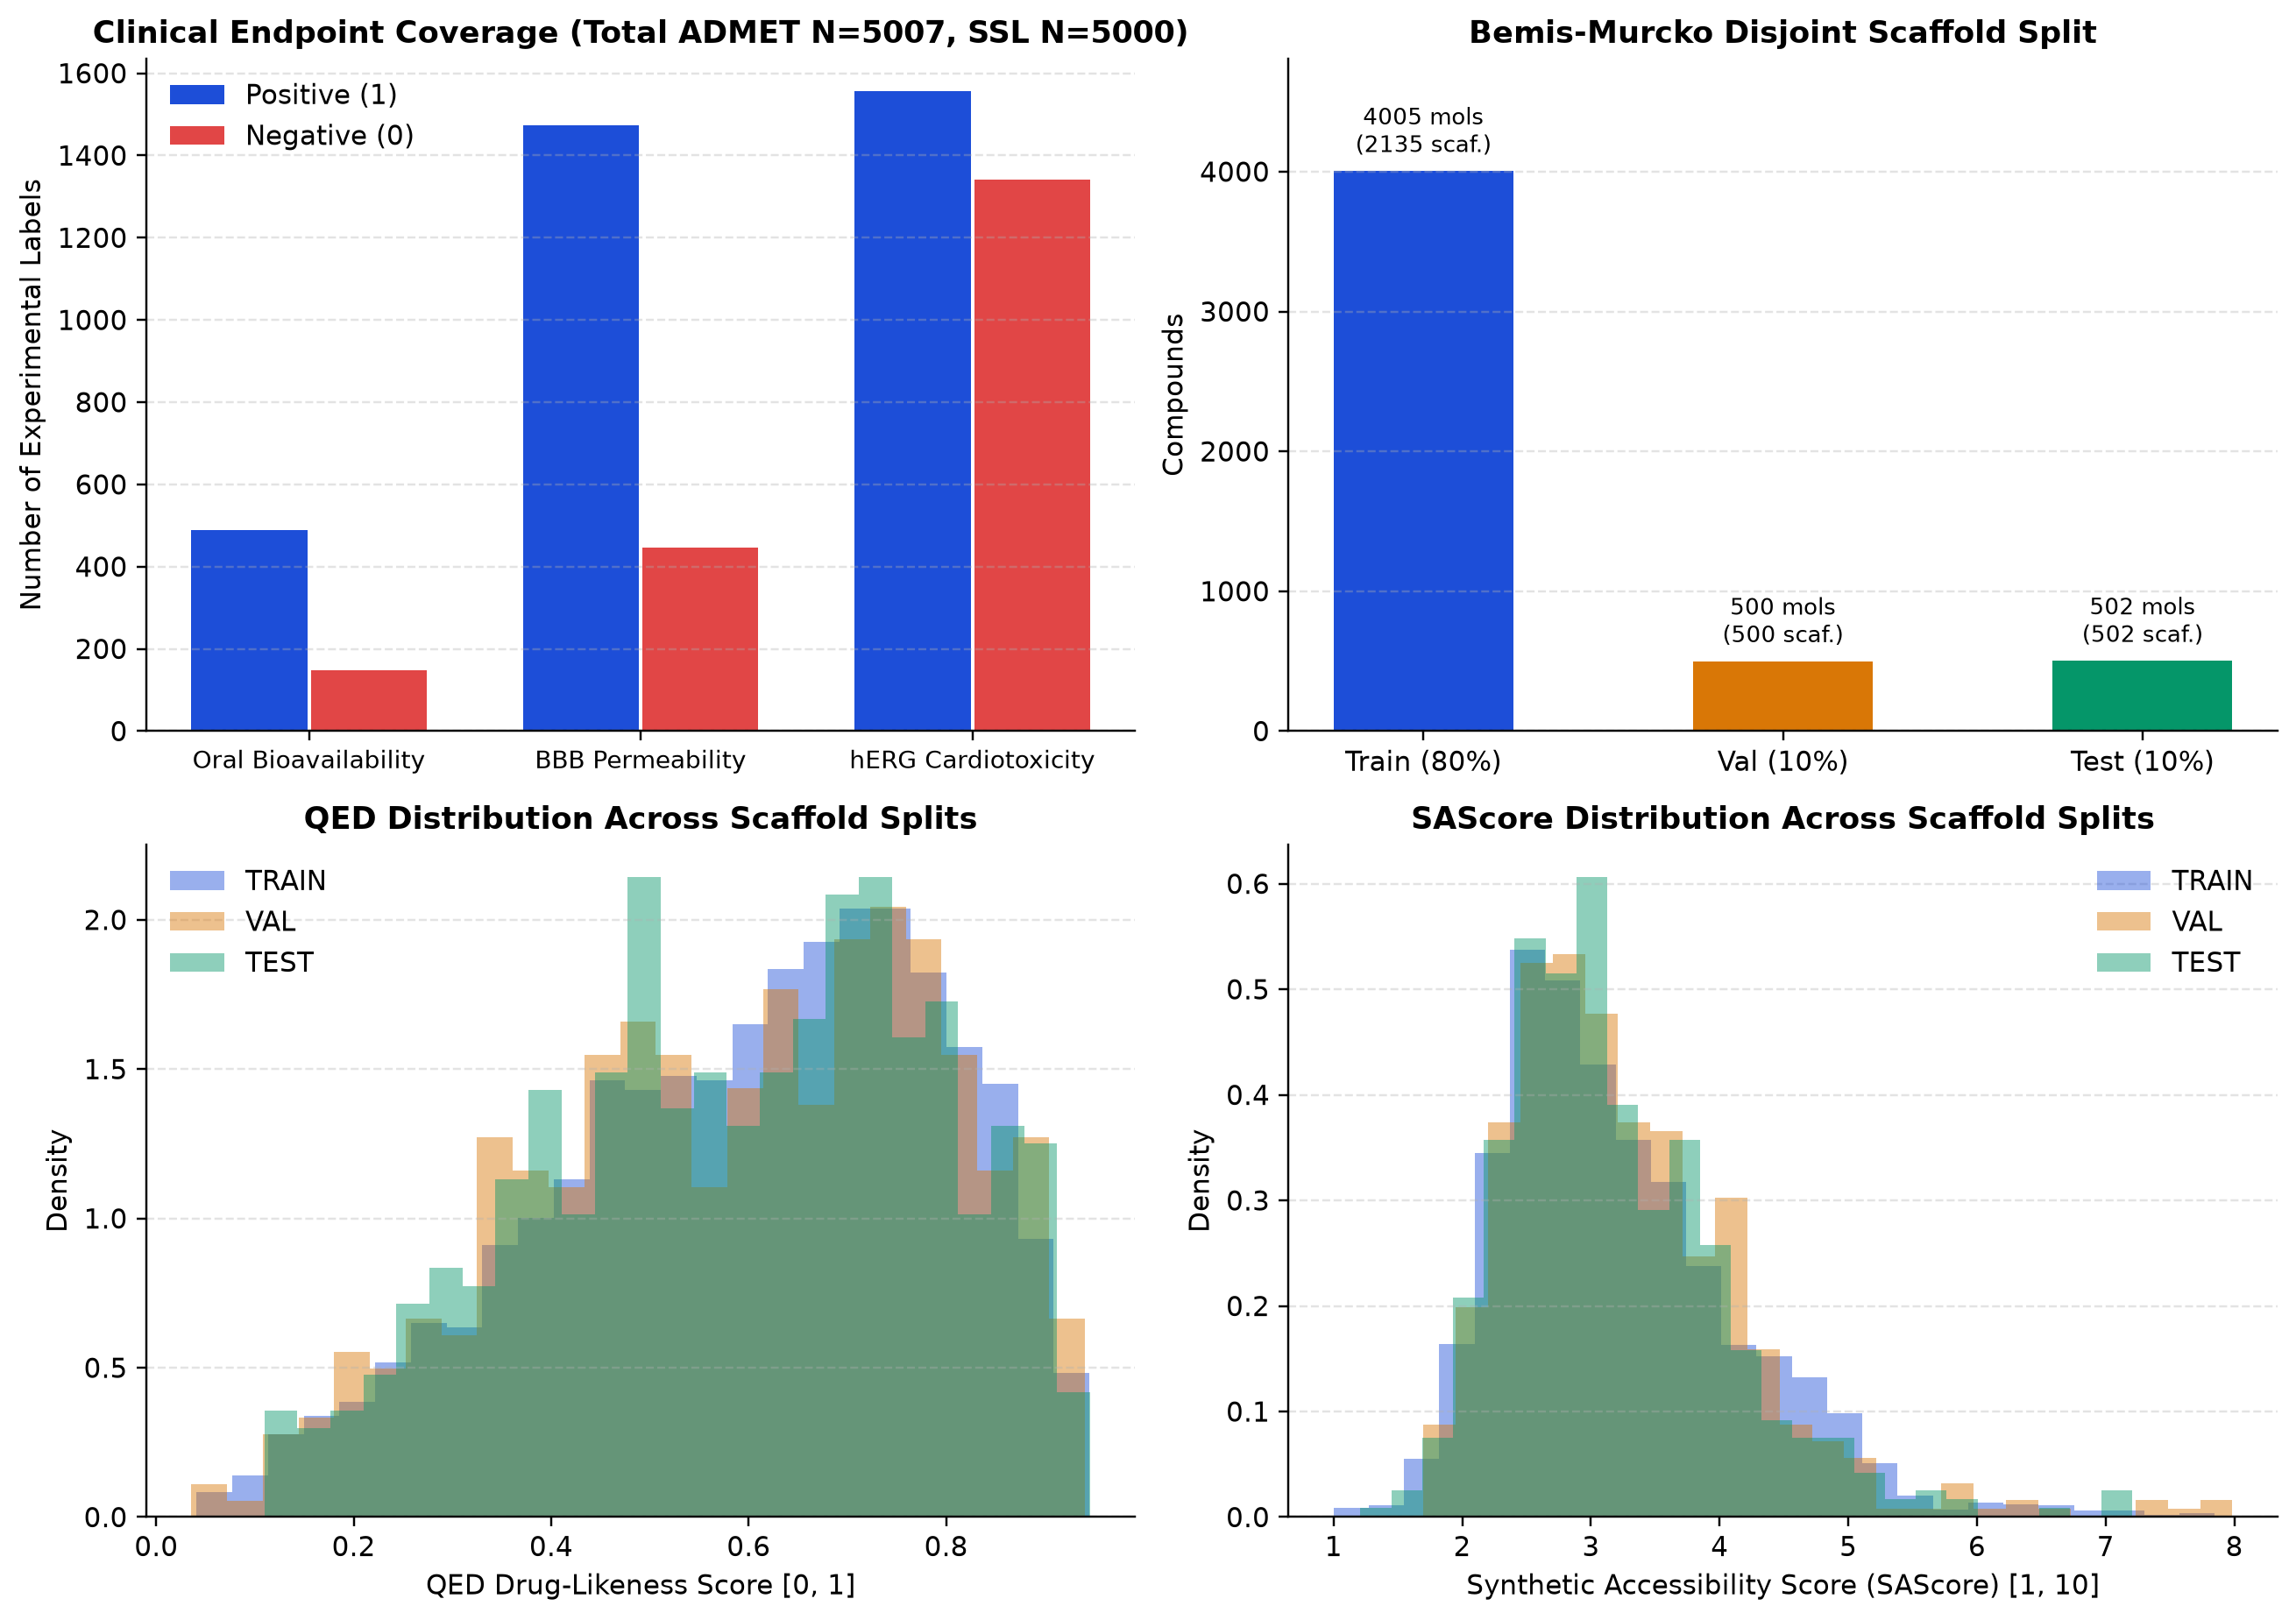
\includegraphics[width=\linewidth]{../results/figures/01_dataset_eda.png}
\caption{Exploratory analysis of curated TDC clinical endpoints, disjoint Bemis-Murcko scaffold split proportions, and QED/SAScore distributions across Train, Validation, and Test splits.}
\label{fig:eda}
\end{figure}

\section{Proposed Methodology}
Figure~\ref{fig:pipeline} illustrates the complete 4-stage pipeline integrating contrastive pre-training, 2D+3D Hybrid GraphGPS encoding, masked multi-task inference, evolutionary Pareto optimization, and explainability.

\begin{figure*}[t]
\centering
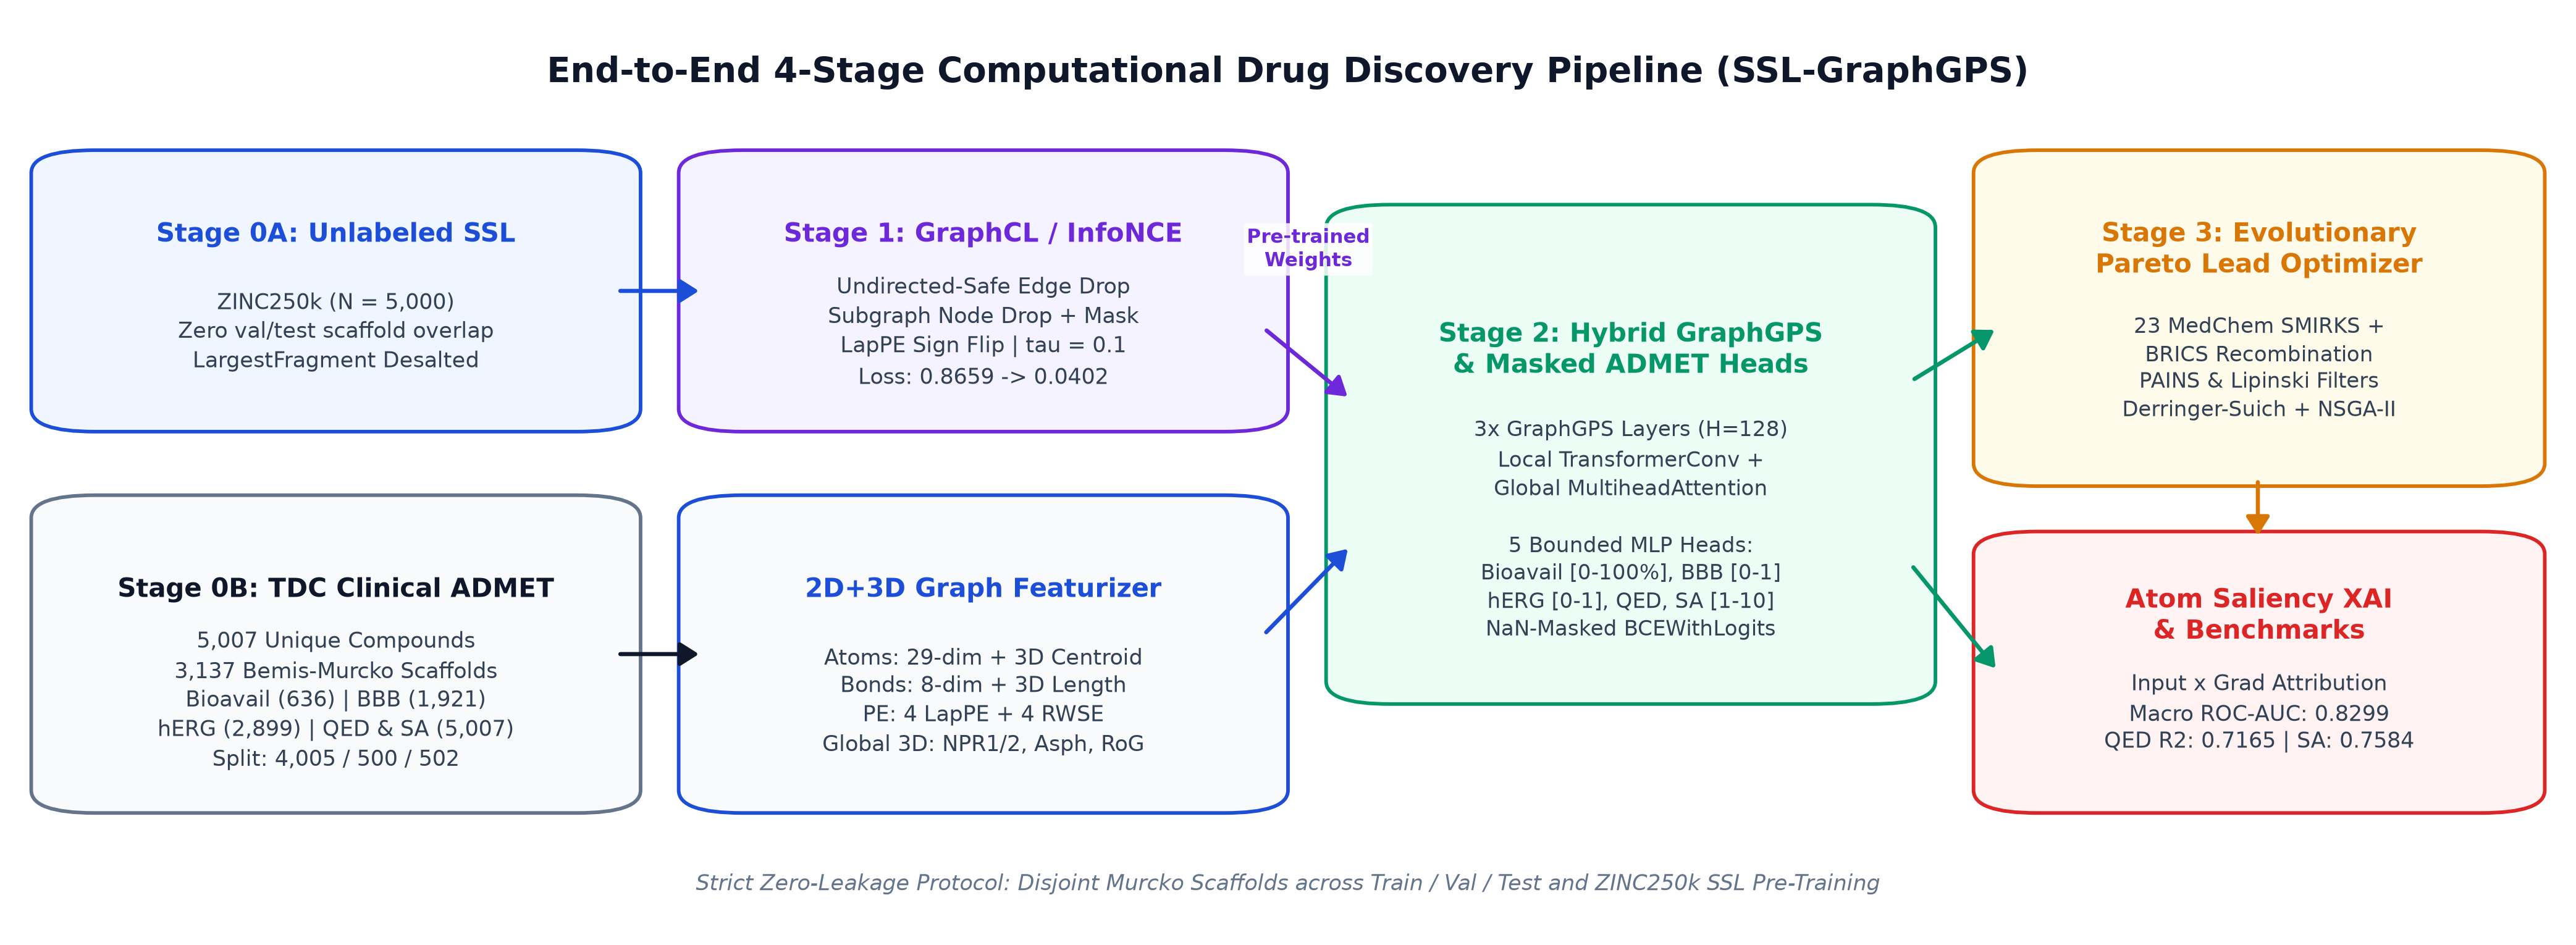
\includegraphics[width=0.94\textwidth]{../results/figures/arch_01_system_pipeline.png}
\caption{End-to-end 4-stage computational drug discovery architecture integrating zero-leakage TDC/ZINC250k curation, GraphCL/InfoNCE self-supervised pre-training, 2D+3D Hybrid GraphGPS ADMET profiling, evolutionary Pareto lead optimization, and atom saliency XAI.}
\label{fig:pipeline}
\end{figure*}

\subsection{2D+3D Graph Featurization and Structural Encodings}
Each desalted molecule is converted into a bidirectional graph $G = (V, E)$. Heavy atoms carry 29-dimensional vectors $x_i \in \mathbb{R}^{29}$ encoding element one-hot (10), total degree (6), formal charge (5, essential for cationic hERG blockers and BBB ionization), hybridization (4), normalized hydrogen count (1), aromaticity (1), ring membership (1), and normalized 3D distance to the heavy-atom centroid (1). Covalent edges carry 8-dimensional vectors $e_{ij} \in \mathbb{R}^8$ capturing bond order/aromaticity (5), conjugation (1), ring flag (1), and 3D bond length (1). Conformer coordinates and global 3D shape descriptors $g_{\text{3D}} = [\text{NPR1}, \text{NPR2}, \text{Asphericity}, \text{RoG}/10] \in \mathbb{R}^4$ are generated via RDKit ETKDGv3 \cite{Riniker2015ETKDG} with deterministic zero fallbacks if embedding fails.

To endow atoms with non-Euclidean topological positions \cite{Dwivedi2022LSPE}, we compute the normalized graph Laplacian $L = I - D^{-1/2} A D^{-1/2}$, filter out trivial zero-eigenvalue modes ($\lambda > 10^{-5}$), and sign-canonicalize the smallest $k=4$ eigenvectors by orienting each column's maximum-magnitude entry to be positive. We concatenate these with 4 sign-invariant Random-Walk Structural Encoding (RWSE) diagonals $\text{diag}(P^1), \dots, \text{diag}(P^4)$ where $P = D^{-1}A$, yielding $p_i \in \mathbb{R}^8$.

\subsection{Hybrid Local+Global 2D+3D GraphGPS Backbone}
Figure~\ref{fig:graphgps} depicts the internal structure of our backbone. Atom features and positional encodings are linearly projected to $H = 128$ and summed ($h^{(0)} = W_x x + W_p p$). Across $L=3$ layers ($4$ attention heads), each layer computes a covalent-edge local attention update \cite{Shi2021TransformerConv} alongside a dense all-atom global self-attention update \cite{Rampasek2022GraphGPS}:
\begin{equation}
h_{\text{loc}}^{(l)} = \text{LN}\!\Big(h^{(l-1)} + \text{Drop}\big(\text{TransformerConv}(h^{(l-1)}, E, W_e e)\big)\Big),
\end{equation}
\begin{equation}
h_{\text{glob}}^{(l)} = \text{LN}\!\Big(h^{(l-1)} + \text{Drop}\big(\text{MHA}_{\text{dense}}(h^{(l-1)}, \text{mask})\big)\Big),
\end{equation}
\begin{equation}
h^{(l)} = \text{LN}\!\Big(\bar{h}^{(l)} + \text{FFN}(\bar{h}^{(l)})\Big), \quad \bar{h}^{(l)} = \frac{1}{2}\big(h_{\text{loc}}^{(l)} + h_{\text{glob}}^{(l)}\big).
\end{equation}
A readout MLP fuses global mean pooling, global max pooling, and projected 3D shape descriptors into a 128-dimensional molecular representation $h_{\text{mol}}$.

\begin{figure}[t]
\centering
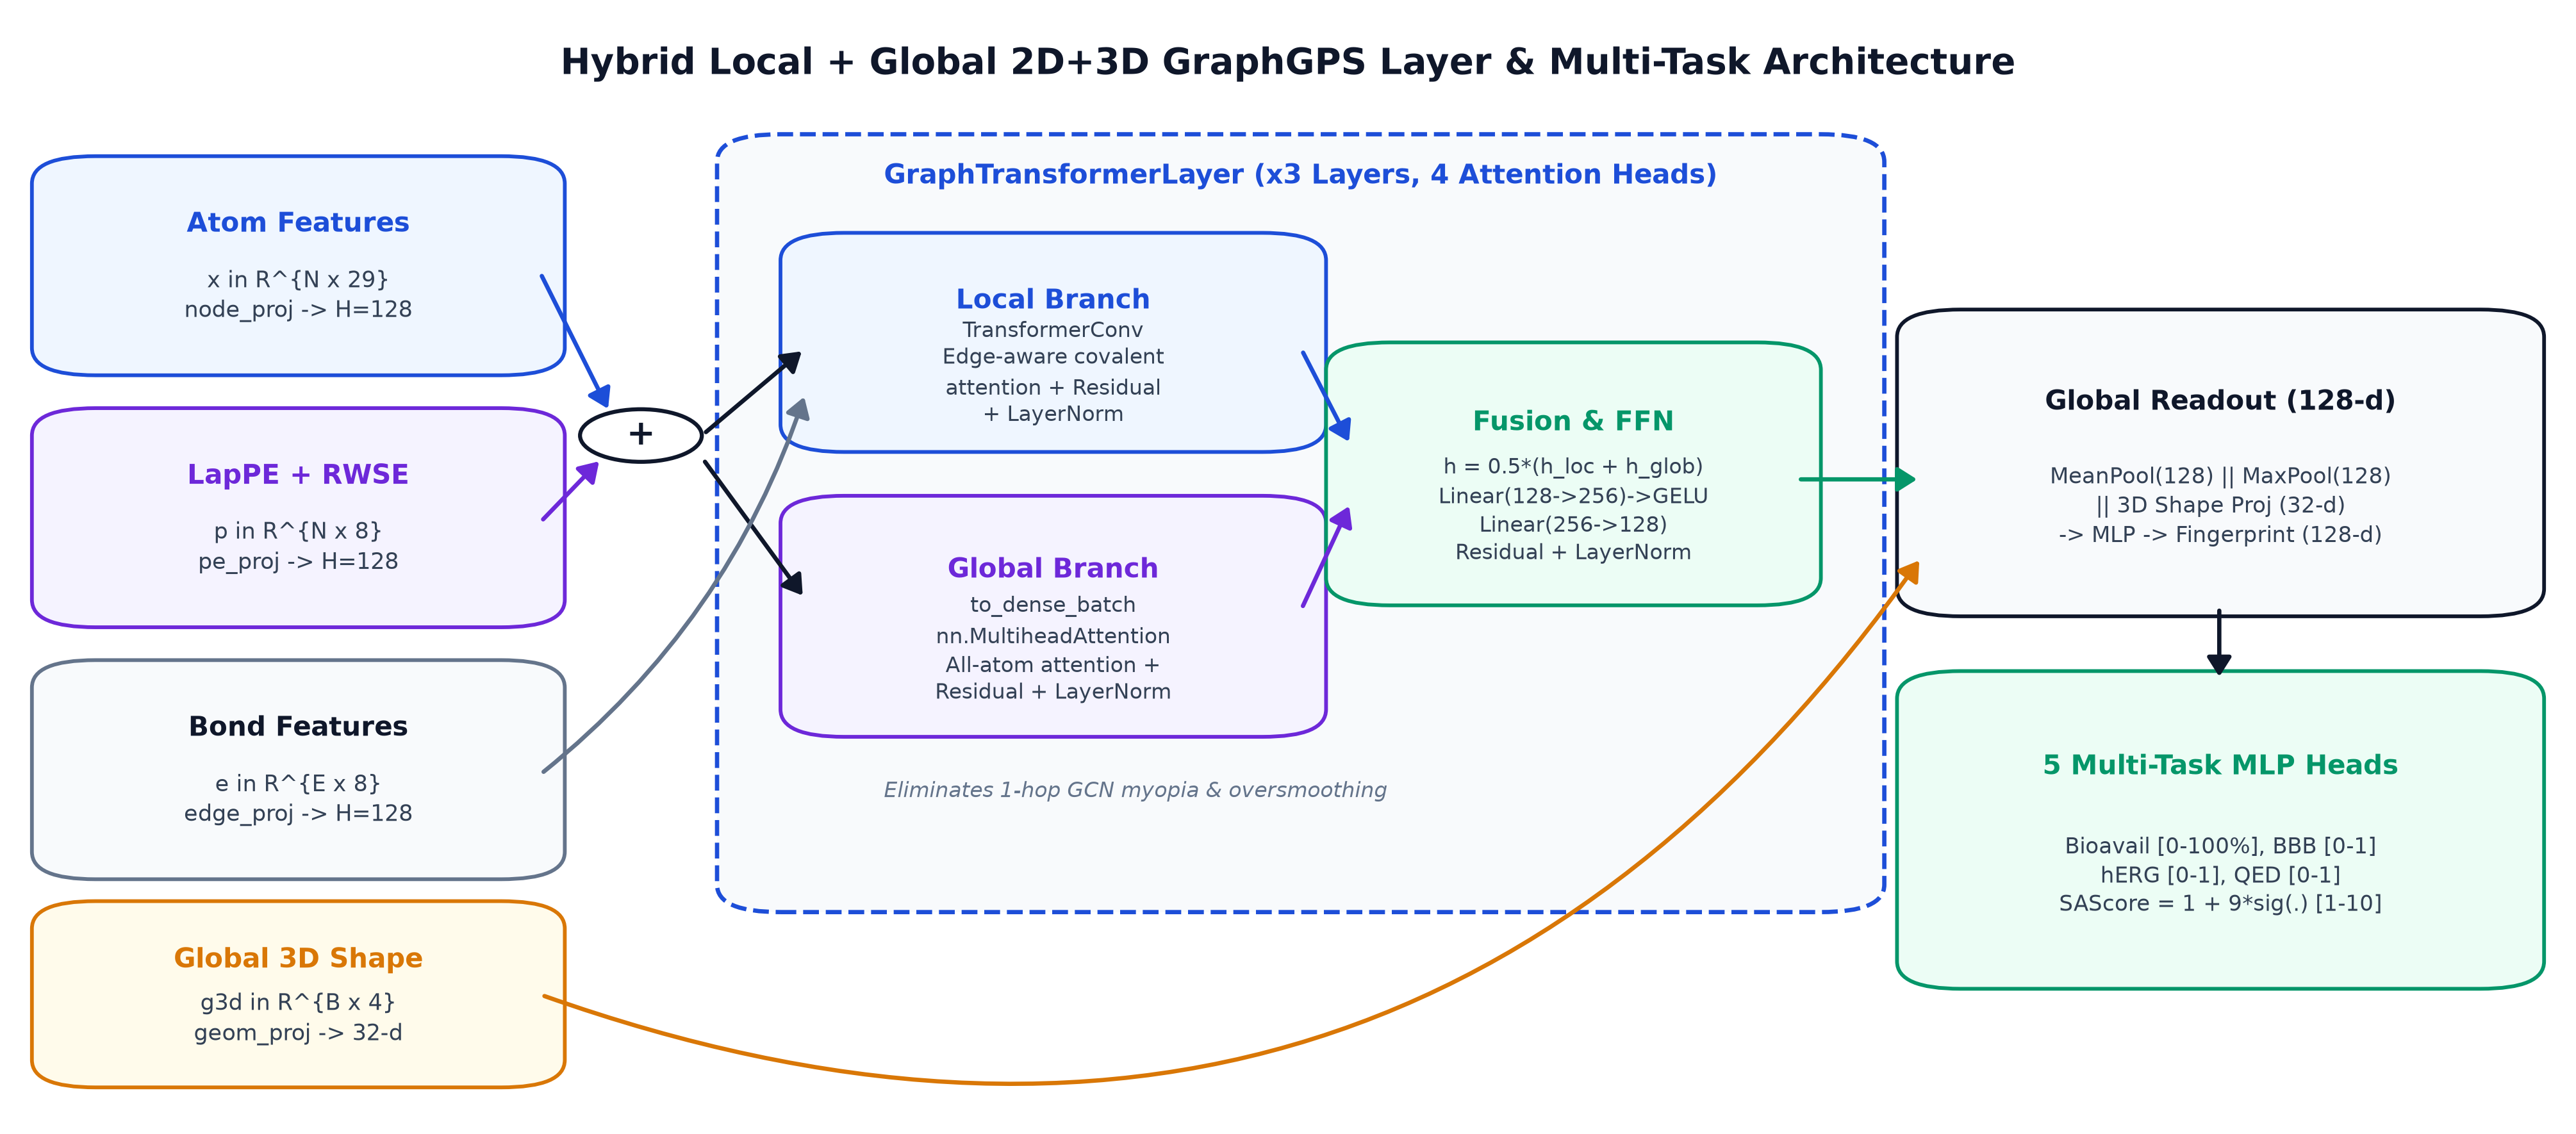
\includegraphics[width=\linewidth]{../results/figures/arch_02_graphgps_layer.png}
\caption{Hybrid Local+Global GraphGPS layer combining edge-aware \texttt{TransformerConv}, dense all-atom \texttt{MultiheadAttention}, and global ETKDGv3 3D shape descriptors.}
\label{fig:graphgps}
\end{figure}

\subsection{Undirected-Safe Contrastive SSL Pre-Training}
Following GraphCL \cite{You2020GraphCL} and MolCLR \cite{Wang2022MolCLR}, each molecule produces two distinct augmented views $(v_i, v_j)$ sampled from atom feature masking (15\%), \emph{undirected-symmetric} bond dropping (15\%, sampling one keep decision per canonical edge $(\min(u,v), \max(u,v))$), subgraph node dropping (15\% with edge remapping), and random LapPE sign flipping. A 2-layer MLP projector with \texttt{BatchNorm1d} maps $h_{\text{mol}}$ to L2-normalized vectors $z_i \in \mathbb{R}^{64}$ trained via temperature-scaled InfoNCE loss ($\tau=0.1$) \cite{Chen2020SimCLR}:
\begin{equation}
\mathcal{L}_{\text{InfoNCE}} = -\log \frac{\exp(\text{sim}(z_i, z_j)/\tau)}{\sum_{k=1}^{2B} \mathbf{1}_{[k \neq i]} \exp(\text{sim}(z_i, z_k)/\tau)}.
\end{equation}

\subsection{Masked Multi-Task ADMET Heads and Bounded Losses}
Task-specific 2-layer MLP heads predict raw logits $(l_{\text{bio}}, l_{\text{bbb}}, l_{\text{herg}})$ mapped via $\sigma(\cdot)$ to $[0,100]\%$ oral bioavailability probability, $[0,1]$ BBB probability, and $[0,1]$ hERG hazard, alongside $\text{QED} \in [0,1]$ and strictly bounded $\text{SAScore} = 1 + 9\sigma(s_{\text{raw}}) \in [1,10]$. Given per-sample boolean mask $M_{i,t} \in \{0,1\}$ indicating observed labels, the joint loss skips missing \texttt{NaN} targets and balances classification and normalized regression scales:
\begin{equation}
\mathcal{L}_{\text{MT}} = \sum_{t \in \{\text{bio},\text{bbb},\text{herg}\}} \mathcal{L}_{\text{BCE}}^{\text{pos\_w}}(l_t, y_t; M_t) + 2\mathcal{L}_{\text{SL1}}(\hat{q}, q) + 2\mathcal{L}_{\text{SL1}}(\hat{\tilde{s}}, \tilde{s}),
\end{equation}
where $\tilde{s} = (s - 1)/9$ normalizes SAScore to $[0, 1]$ and $\text{pos\_w} = \text{clip}(N_{\text{neg}}/N_{\text{pos}}, 0.5, 4.0)$ is computed strictly on the training split.

\subsection{Evolutionary Pareto Lead Optimization and Atom Saliency}
Starting from a seed lead, our mutator applies 23 warning-free medicinal chemistry reaction SMIRKS (aromatic/aliphatic substitutions, aza-scans, halogen swaps, carboxylic bioisosteres) plus RDKit BRICS fragment recombination \cite{Degen2008BRICS}, retaining only molecules passing PAINS alerts \cite{Baell2010PAINS}, Lipinski Ro5 ($\le 1$ violation) \cite{Lipinski2001Ro5}, and Tanimoto ECFP4 similarity $\ge 0.35$ \cite{Rogers2010ECFP}. Candidates are scored using the Derringer-Suich geometric desirability function \cite{Derringer1980Desirability}:
\begin{equation}
D(x) = \left( d_{\text{bio}}^{w_1} \cdot d_{1-\text{hERG}}^{w_2} \cdot d_{\text{QED}}^{w_3} \cdot d_{\text{SA}}^{w_4} \cdot d_{\text{BBB}}^{w_5} \right)^{1/\sum_{j=1}^5 w_j},
\end{equation}
with $(w_1,\dots,w_5) = (1.0, 1.5, 1.0, 0.8, 0.4)$ and $d_{\text{BBB}} = 1 - \text{BBB}$ in \texttt{peripheral} mode (penalizing unwanted CNS exposure), and ranked into non-dominated fronts via NSGA-II peeling \cite{Deb2002NSGA2}. Finally, atom-level attribution \cite{Shrikumar2017InputGrad} computes normalized sensitivity scores per atom $i$ as:
\begin{equation}
A_i = \sqrt{\sum_{d=1}^{29} \left(x_{i,d} \cdot \frac{\partial l_{\text{task}}}{\partial x_{i,d}}\right)^2}.
\end{equation}

\section{Experimental Setup and Ablation Results}
\subsection{Training Hyperparameters and Baselines}
All experiments use deterministic seed \texttt{42}, Apple Silicon MPS acceleration, \texttt{AdamW} ($\text{wd}=10^{-4}$), cosine LR annealing ($\eta_{\min}=10^{-5}$), gradient norm clipping ($1.0$), and batch size 64. Stage~1 SSL pre-trains for 25 epochs ($\text{lr}=10^{-3}$). Stage~2 fine-tuning runs up to 40 epochs ($\text{lr}=5\times 10^{-4}$, discriminative $0.5\times$ backbone LR for SSL initialization) with validation early stopping ($\text{patience}=10$) maximizing $0.7\cdot\text{Macro-ROC-AUC} + 0.3\cdot\overline{R^2}$. We compare four models identically on the unseen-scaffold test split ($n=502$): (1) \textbf{RF-ECFP4} (300 balanced trees per task on 2048-bit Morgan ECFP4 \cite{Rogers2010ECFP,Breiman2001RF}), (2) \textbf{Standard-GCN} (3-layer \texttt{GCNConv} \cite{Kipf2017GCN} with identical 5-task heads), (3) \textbf{GraphGPS-Scratch} (no SSL pre-training), and (4) \textbf{SSL-GraphGPS (Ours)}.

\subsection{Stage 1 Contrastive Convergence and Latent Organization}
InfoNCE loss decreased monotonically from \textbf{0.8659} (epoch 1) to \textbf{0.1218} (epoch 5), \textbf{0.0644} (epoch 10), and \textbf{0.0408} at epoch 25 (best checkpoint \textbf{0.0402}). Figure~\ref{fig:ssl} shows smooth zero-shot latent clustering along QED drug-likeness and partial unsupervised separation of hERG-toxic scaffolds across validation and test compounds prior to seeing any clinical labels.

\begin{figure}[t]
\centering
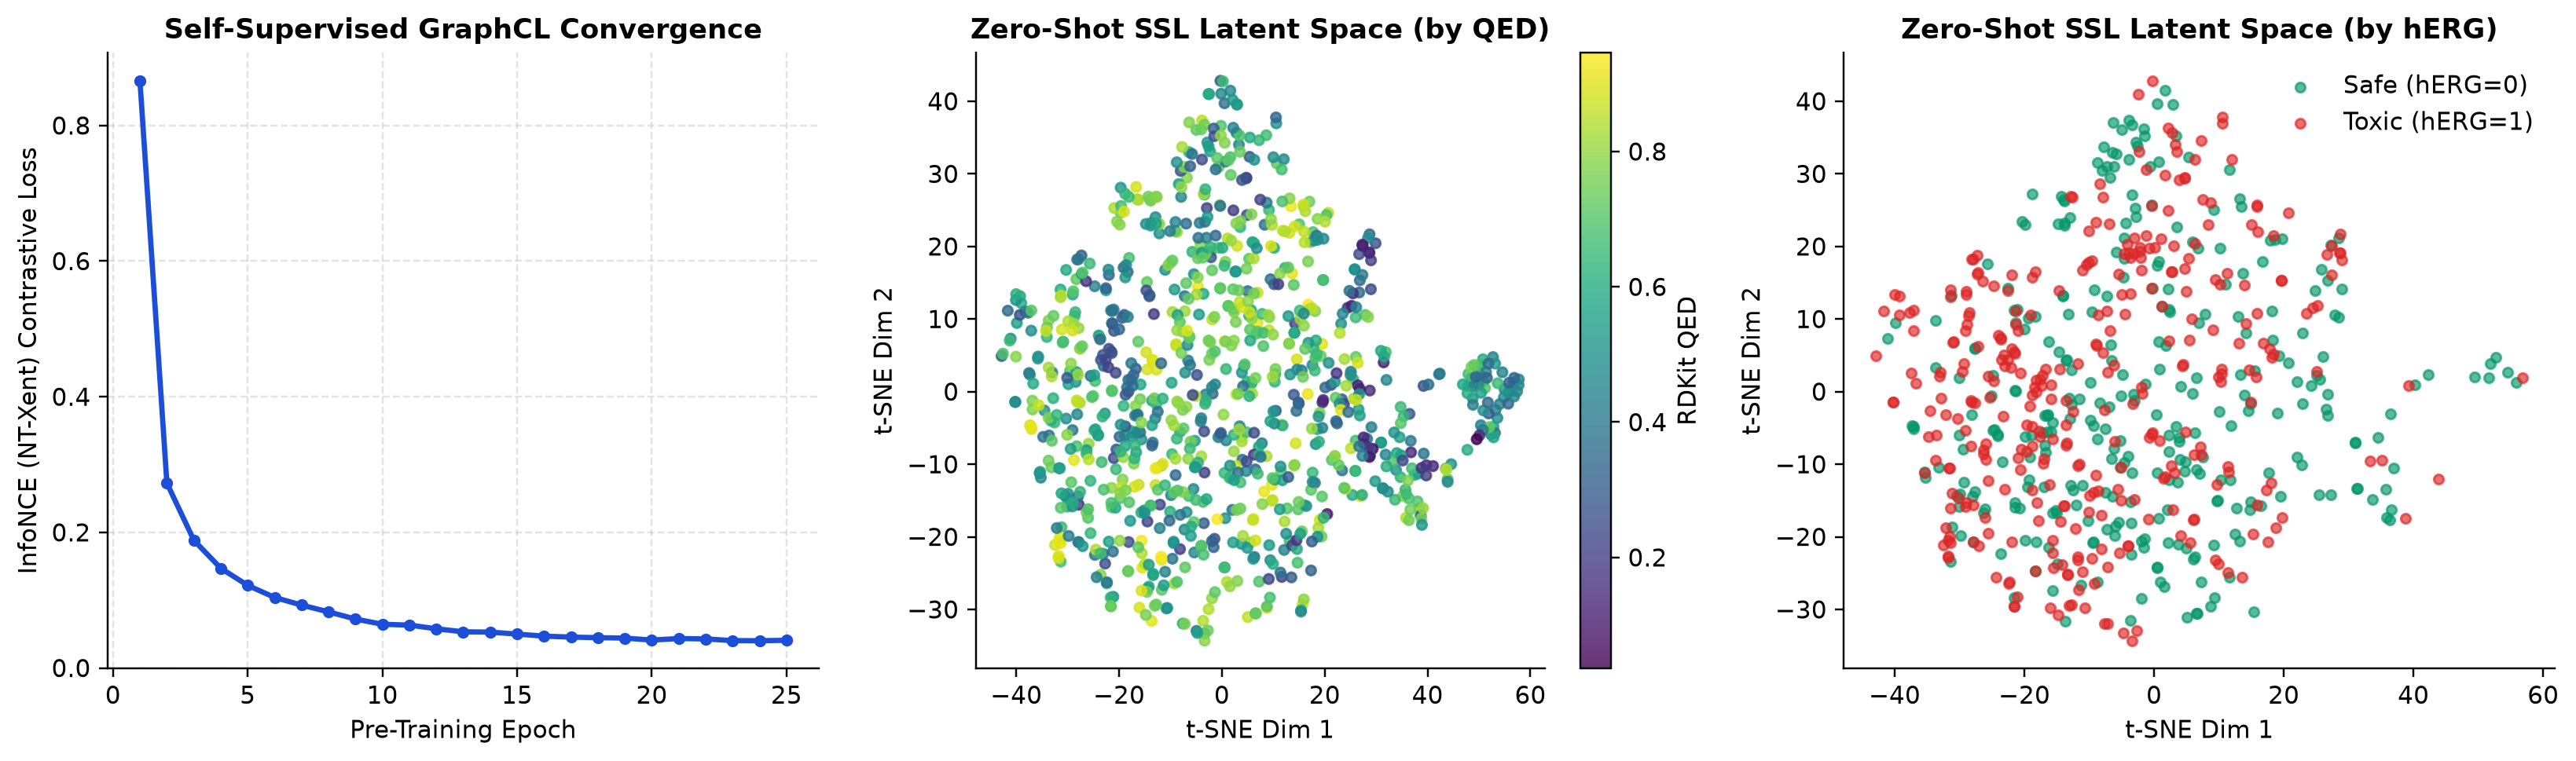
\includegraphics[width=\linewidth]{../results/figures/02_ssl_pretraining.png}
\caption{Stage 1 SSL InfoNCE convergence across 25 epochs on 5,000 ZINC250k molecules (left) and zero-shot t-SNE latent representations on unseen val/test scaffolds colored by QED (center) and hERG hazard (right).}
\label{fig:ssl}
\end{figure}

\subsection{Held-Out Unseen-Scaffold Benchmark and Ablation}
Table~\ref{tab:benchmark} and Figs.~\ref{fig:curves}--\ref{fig:parity} summarize the held-out unseen-scaffold evaluation. \textbf{SSL-GraphGPS} achieves the strongest performance on \textbf{every single endpoint}: \textbf{0.8299 Macro ROC-AUC} (Bioavailability 0.7769 / PR-AUC 0.9089; BBB 0.9001 / PR-AUC 0.9728; hERG 0.8128 / PR-AUC 0.8016), \textbf{$R^2=0.7165$} on QED ($\text{MAE}=0.082$, Pearson $r=0.8465$), and \textbf{$R^2=0.7584$} on SAScore ($\text{MAE}=0.324$, Pearson $r=0.8774$).

Comparing \textbf{SSL-GraphGPS} against \textbf{GraphGPS-Scratch} quantifies the direct benefit of contrastive pre-training: \textbf{+3.43 percentage points (pp) in Macro ROC-AUC}, led by a \textbf{+7.17 pp} gain on data-scarce Oral Bioavailability ($n_{\text{train}}=536$), +1.97 pp on hERG, +1.18 pp on BBB, +0.023 on QED $R^2$, and +0.074 on SAScore $R^2$. Comparing against \textbf{Standard-GCN} highlights the expressive advantage of hybrid 2D+3D local-global attention (+2.33 pp Macro ROC-AUC and +0.347 QED $R^2$).

\begin{table*}[t]
\centering
\caption{Held-Out Unseen-Scaffold Test Benchmark ($n = 502$, Zero Scaffold or SMILES Overlap with Training/SSL)}
\label{tab:benchmark}
\begin{tabular}{lccccccc}
\toprule
\textbf{Model} & \textbf{Bioavail. AUC} & \textbf{BBB AUC} & \textbf{hERG AUC} & \textbf{Macro ROC-AUC} & \textbf{QED $R^2$ (MAE)} & \textbf{SAScore $R^2$ (MAE)} & \textbf{Comp. Score} \\
\midrule
RF-ECFP4 \cite{Rogers2010ECFP,Breiman2001RF} & 0.7658 & 0.8758 & 0.7794 & 0.8070 & 0.5612 (0.101) & 0.7341 (\textbf{0.317}) & 0.7592 \\
Standard-GCN \cite{Kipf2017GCN}              & 0.7466 & 0.8945 & 0.7786 & 0.8066 & 0.3699 (0.127) & 0.6044 (0.421) & 0.7107 \\
GraphGPS-Scratch (Ablation)                  & 0.7052 & 0.8883 & 0.7931 & 0.7956 & 0.6935 (0.087) & 0.6844 (0.380) & 0.7636 \\
\textbf{SSL-GraphGPS (Ours)}                 & \textbf{0.7769} & \textbf{0.9001} & \textbf{0.8128} & \textbf{0.8299} & \textbf{0.7165 (0.082)} & \textbf{0.7584} (0.324) & \textbf{0.8022} \\
\midrule
\emph{SSL Gain vs. Scratch} & \emph{+0.0717} & \emph{+0.0118} & \emph{+0.0197} & \emph{+0.0343} & \emph{+0.0230} & \emph{+0.0740} & \emph{+0.0386} \\
\bottomrule
\end{tabular}
\end{table*}

\begin{figure}[t]
\centering
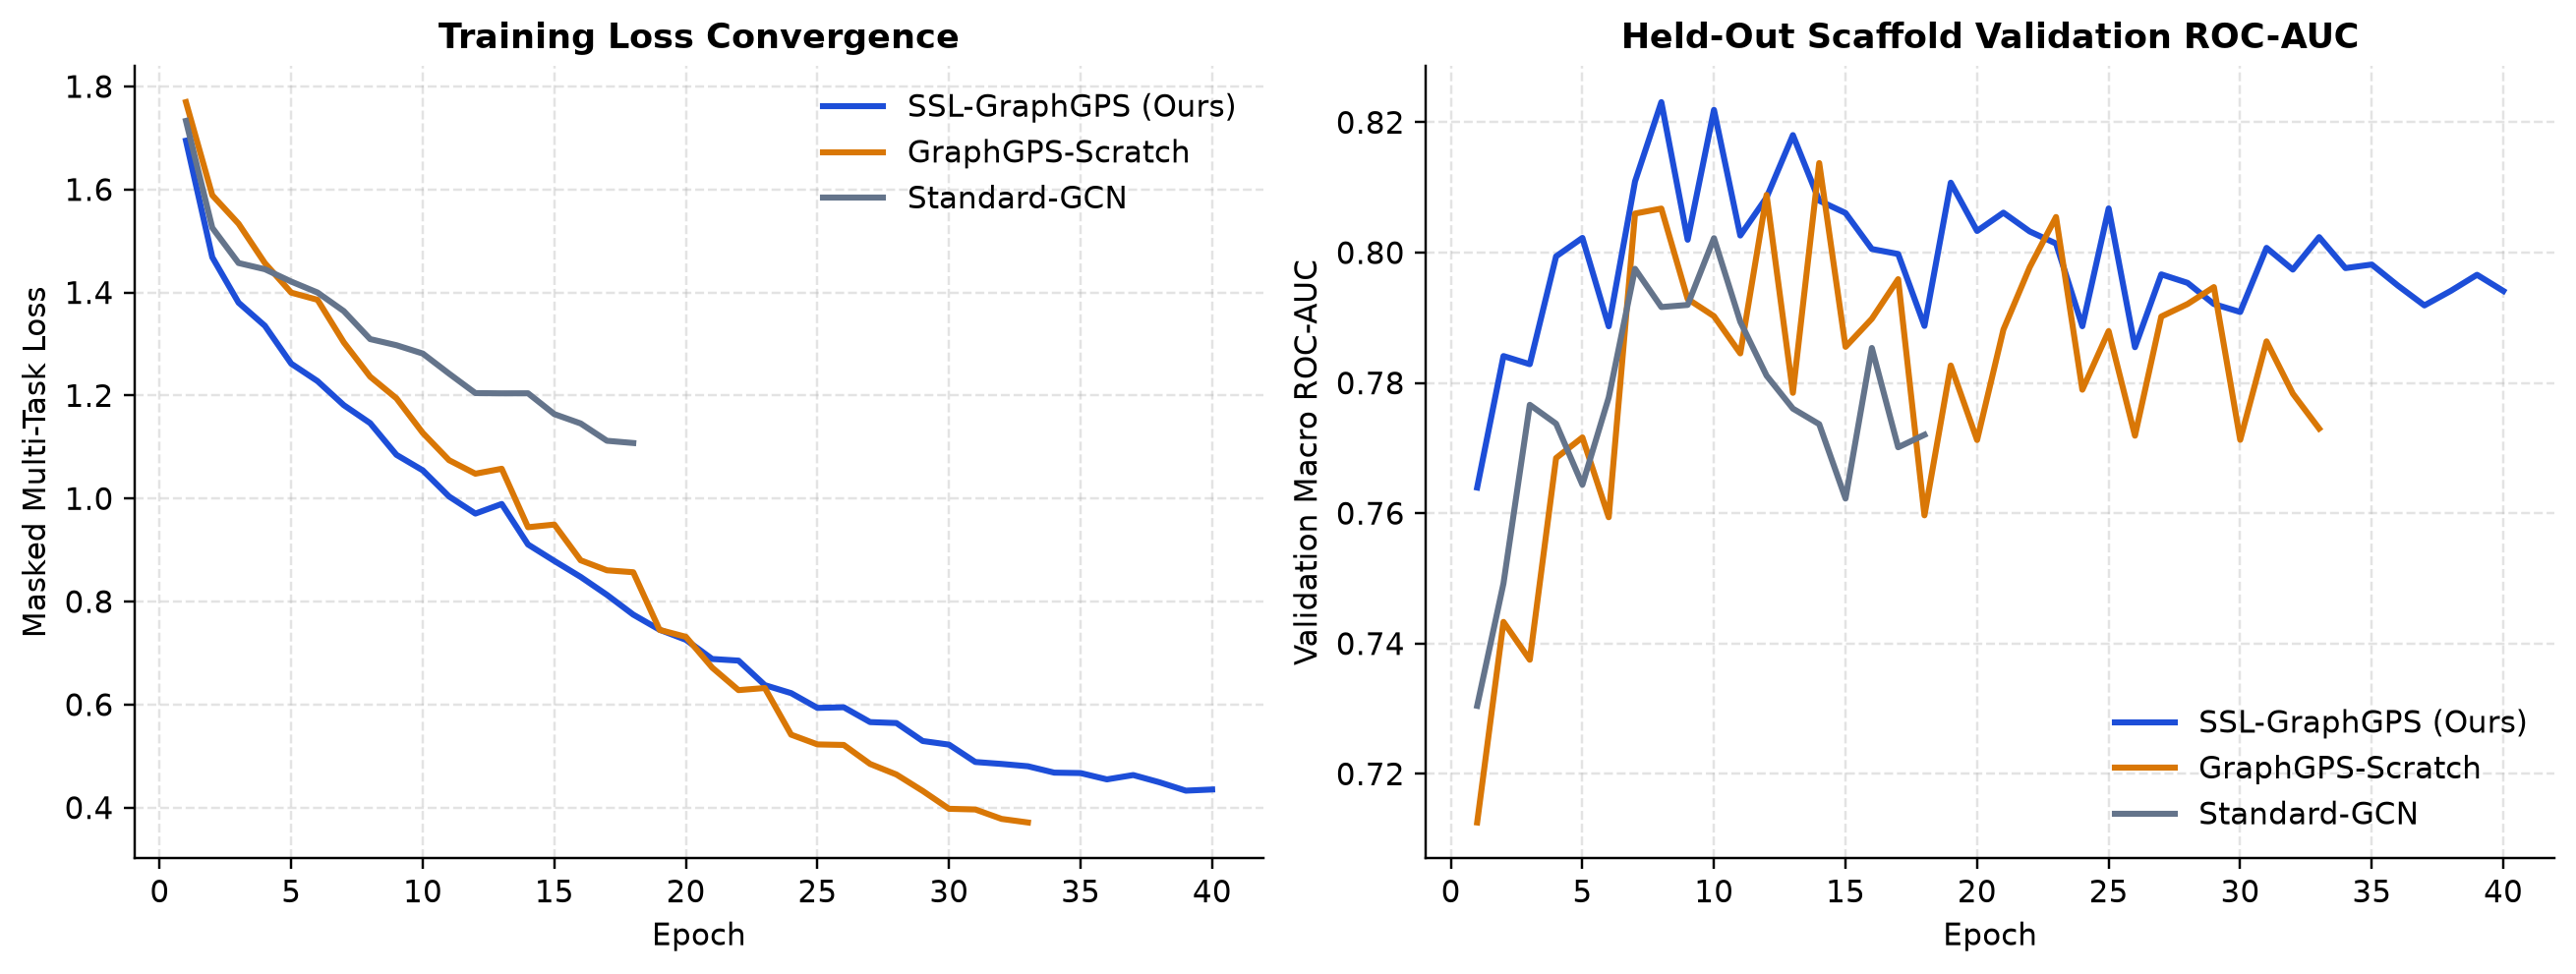
\includegraphics[width=\linewidth]{../results/figures/03_training_curves.png}
\caption{Training loss convergence and unseen-scaffold validation Macro ROC-AUC across SSL-GraphGPS, GraphGPS-Scratch, and Standard-GCN.}
\label{fig:curves}
\end{figure}

\begin{figure*}[t]
\centering
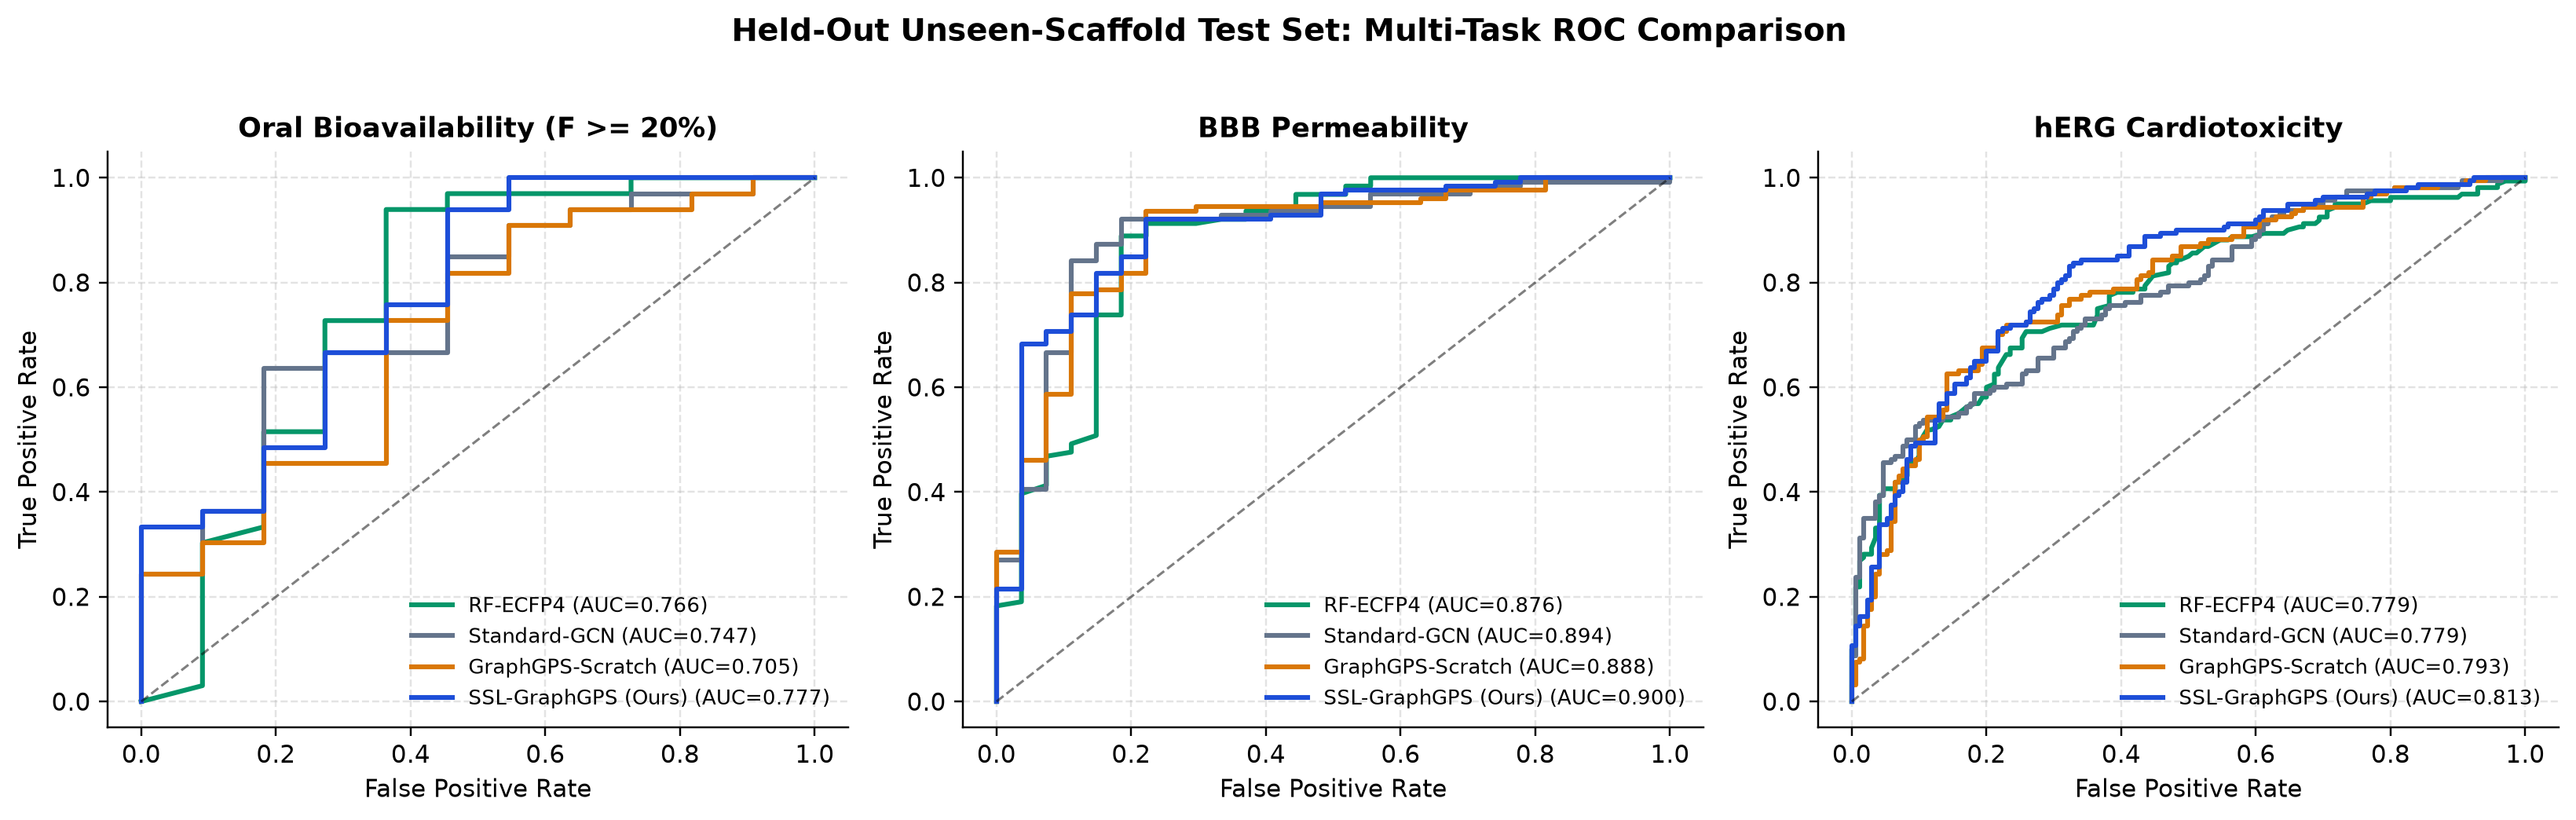
\includegraphics[width=0.92\textwidth]{../results/figures/04_roc_comparison.png}
\caption{Held-out unseen-scaffold ROC curve comparison across Oral Bioavailability ($n=44$), BBB Permeability ($n=153$), and hERG Cardiotoxicity ($n=330$).}
\label{fig:roc}
\end{figure*}

\begin{figure}[t]
\centering
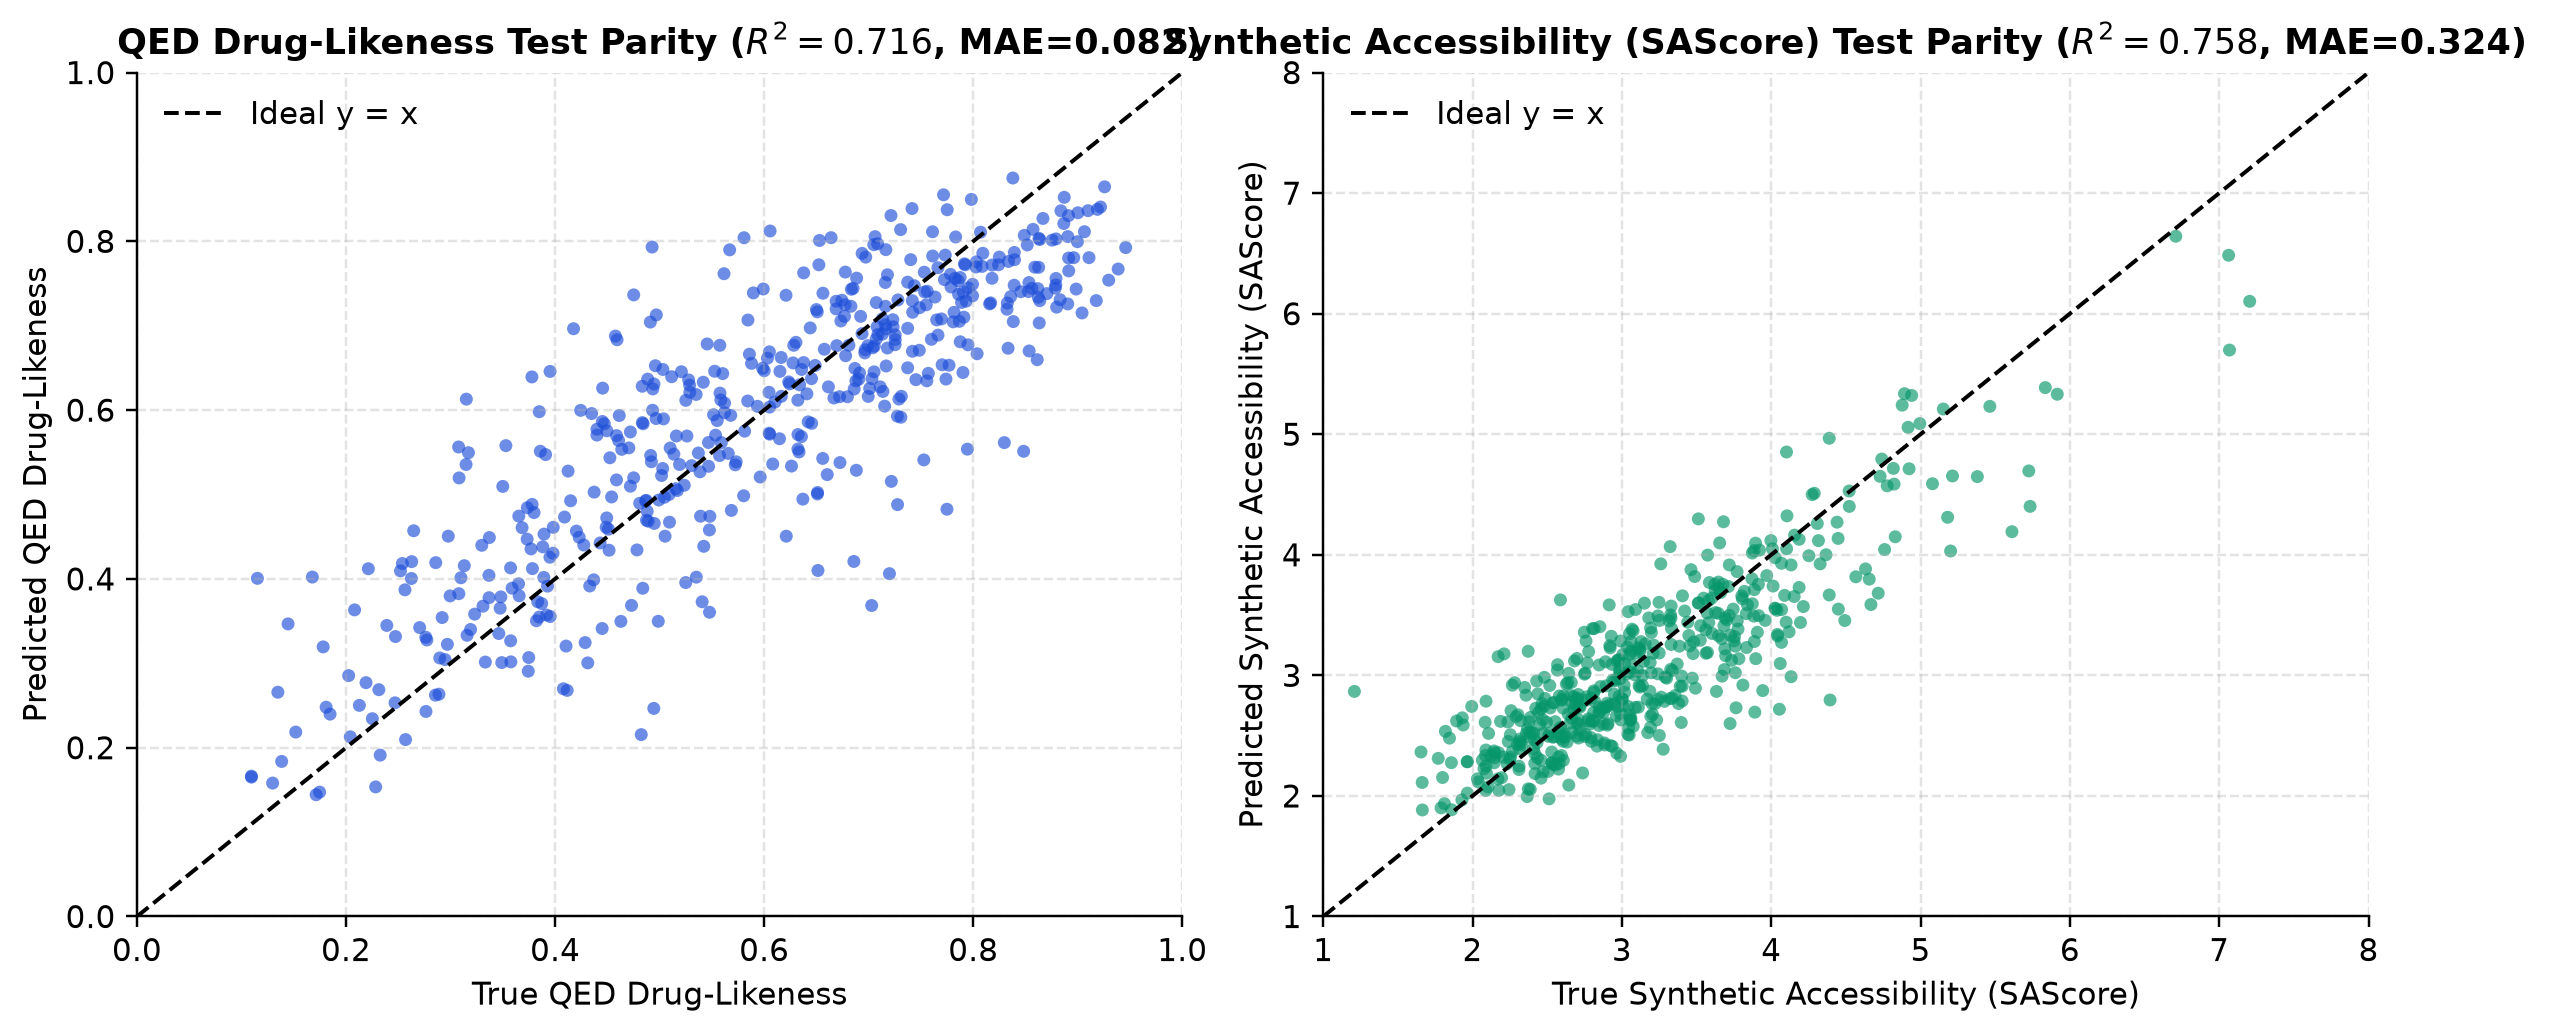
\includegraphics[width=\linewidth]{../results/figures/05_regression_parity.png}
\caption{Predicted vs. ground-truth test parity plots for SSL-GraphGPS on QED ($R^2=0.7165$) and SAScore ($R^2=0.7584$).}
\label{fig:parity}
\end{figure*}

\section{Lead Optimization Case Study and Explainability}
Applying two evolutionary generations around \textbf{Aspirin} (\texttt{CC(=O)Oc1ccccc1C(=O)O}) in \texttt{peripheral} mode explored \textbf{70 PAINS-free, Lipinski-compliant analogues} ($T \ge 0.35$) and identified \textbf{45 non-dominated Pareto Front-1 solutions} (Table~\ref{tab:leadopt} and Fig.~\ref{fig:pareto}). Top Front-1 analogues increase composite desirability from 0.898 (seed) to \textbf{0.919} while lowering predicted unwanted CNS exposure ($\text{BBB}: 0.216 \to 0.037\text{--}0.081$), preserving ultra-low hERG risk ($\le 0.013$), and raising exact RDKit QED from 0.550 to 0.644.

\begin{table}[t]
\centering
\caption{Aspirin Multi-Generation Pareto Front-1 Lead Optimization}
\label{tab:leadopt}
\setlength{\tabcolsep}{3.2pt}
\begin{tabular}{lcccccc}
\toprule
\textbf{Candidate} & \textbf{Bio\%} & \textbf{hERG} & \textbf{BBB} & \textbf{QED(P/RD)} & \textbf{SA(P/RD)} & \textbf{Desir.} \\
\midrule
Seed (Aspirin)     & 99.9 & 0.004 & 0.216 & 0.74/0.55 & 2.06/1.58 & 0.898 \\
\textbf{\#1 Di-Et} & 100.0 & 0.005 & 0.081 & 0.78/0.64 & 2.15/2.15 & \textbf{0.919} \\
\textbf{\#2 4-Et}  & 99.9  & 0.003 & 0.043 & 0.76/0.61 & 2.13/1.81 & \textbf{0.917} \\
\textbf{\#3 4-Me}  & 99.8  & 0.005 & 0.037 & 0.76/0.57 & 2.13/1.76 & \textbf{0.916} \\
\textbf{\#4 Me,Cl} & 100.0 & 0.013 & 0.041 & 0.78/0.62 & 2.27/1.97 & \textbf{0.916} \\
\textbf{\#5 4-Cl}  & 99.7  & 0.006 & 0.032 & 0.75/0.60 & 2.16/1.73 & \textbf{0.915} \\
\bottomrule
\end{tabular}
\end{table}

\begin{figure}[t]
\centering
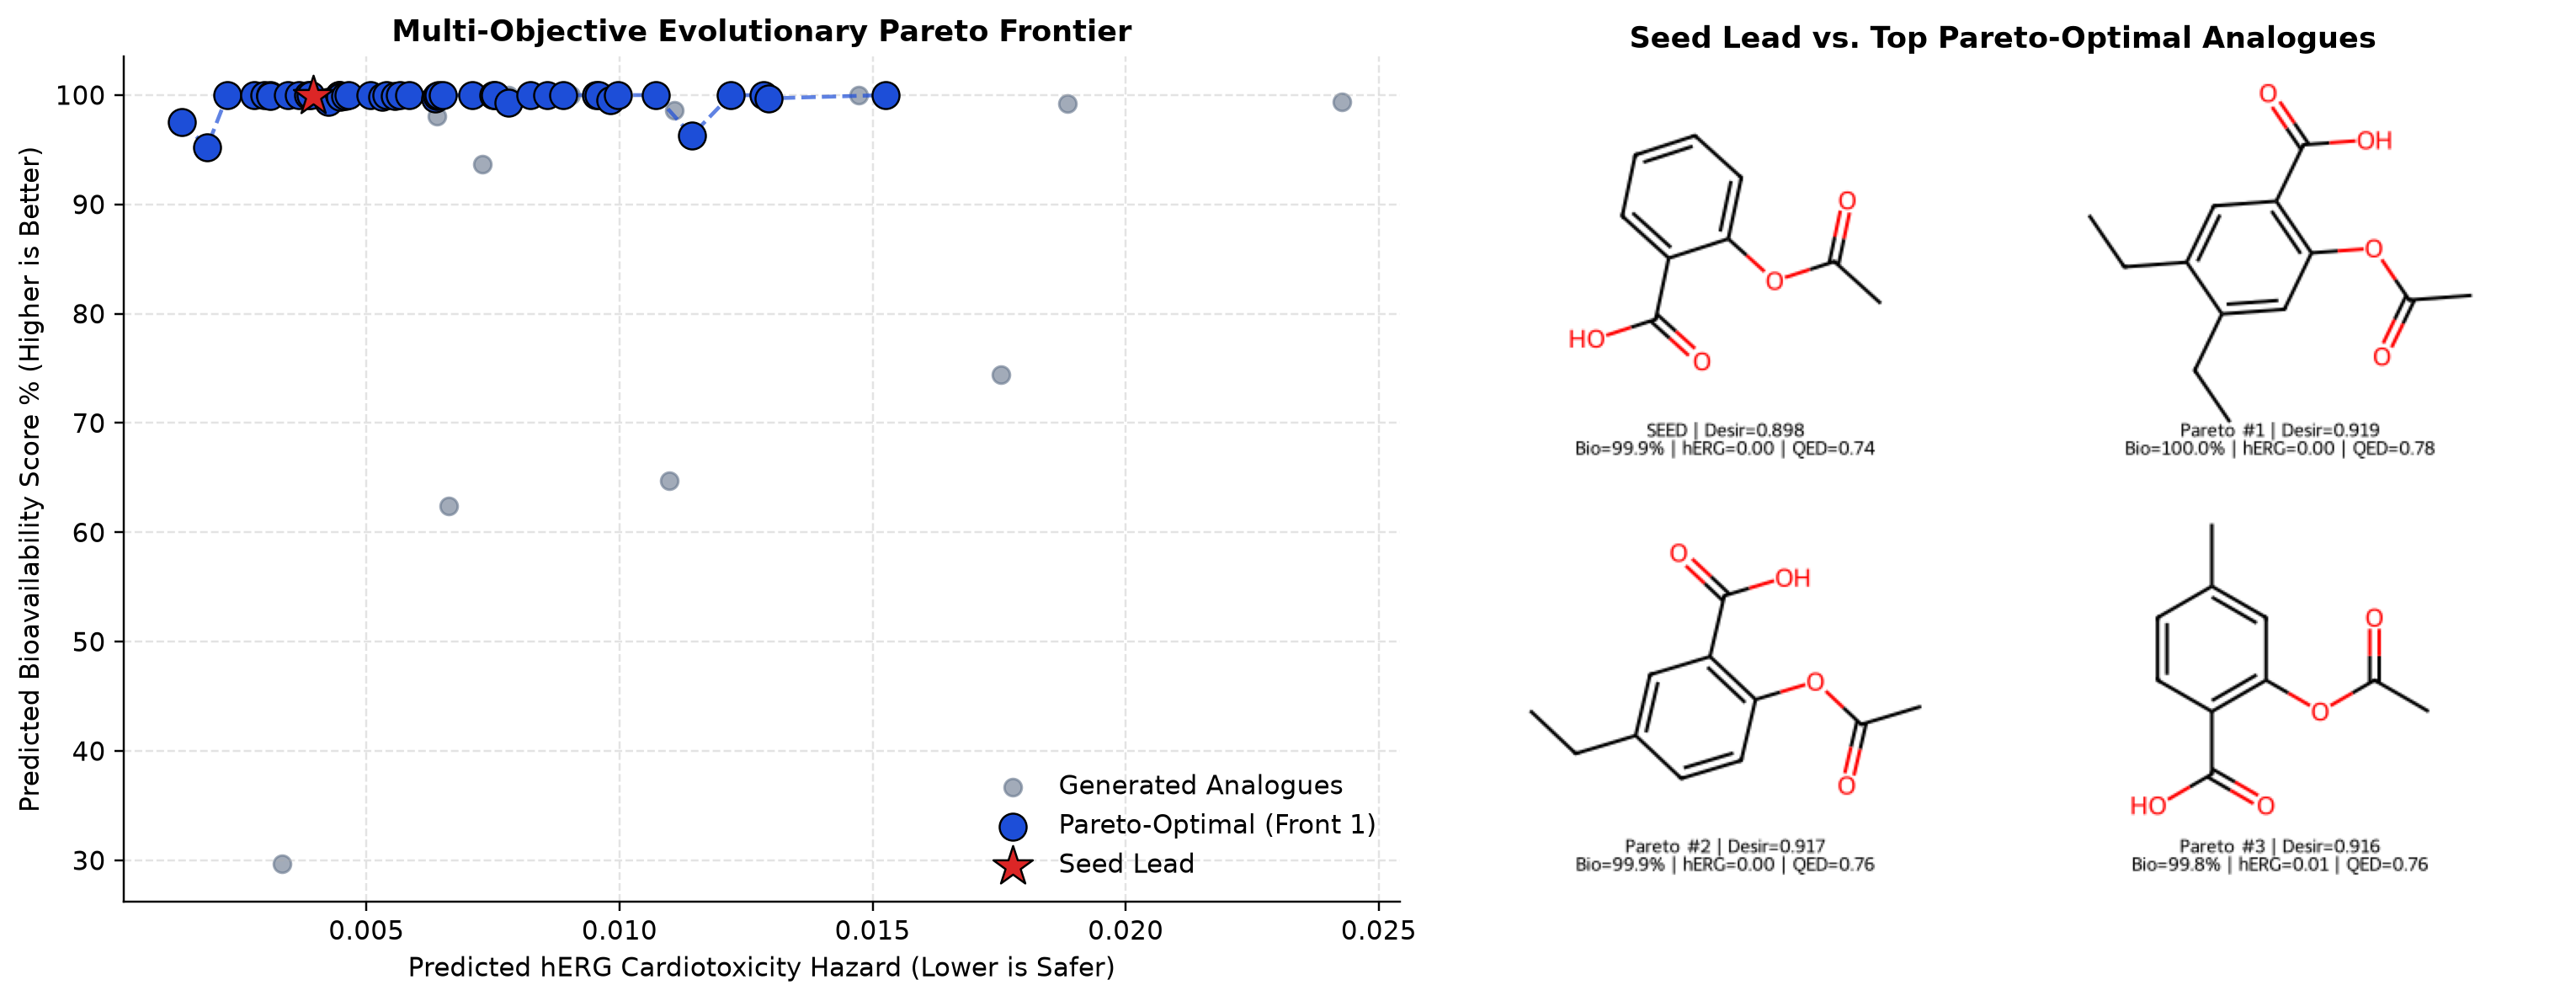
\includegraphics[width=\linewidth]{../results/figures/06_pareto_optimization.png}
\caption{Bioavailability vs. hERG Pareto Front-1 scatter (left) and 2D structures of Aspirin seed vs. top Pareto-optimal analogues (right).}
\label{fig:pareto}
\end{figure}

Figure~\ref{fig:xai} visualizes atom-level gradient attribution across an unseen test-set hERG blocker ($\text{pred}=0.996$), Aspirin ($\text{hERG}=0.004$), and Caffeine ($\text{BBB}=0.941$). On the unseen hERG blocker, saliency concentrates on the protonatable tertiary amine nitrogen and adjacent linker carbons---consistent with classic hERG potassium channel binding pharmacophores \cite{Wang2016hERG}.

\begin{figure}[t]
\centering
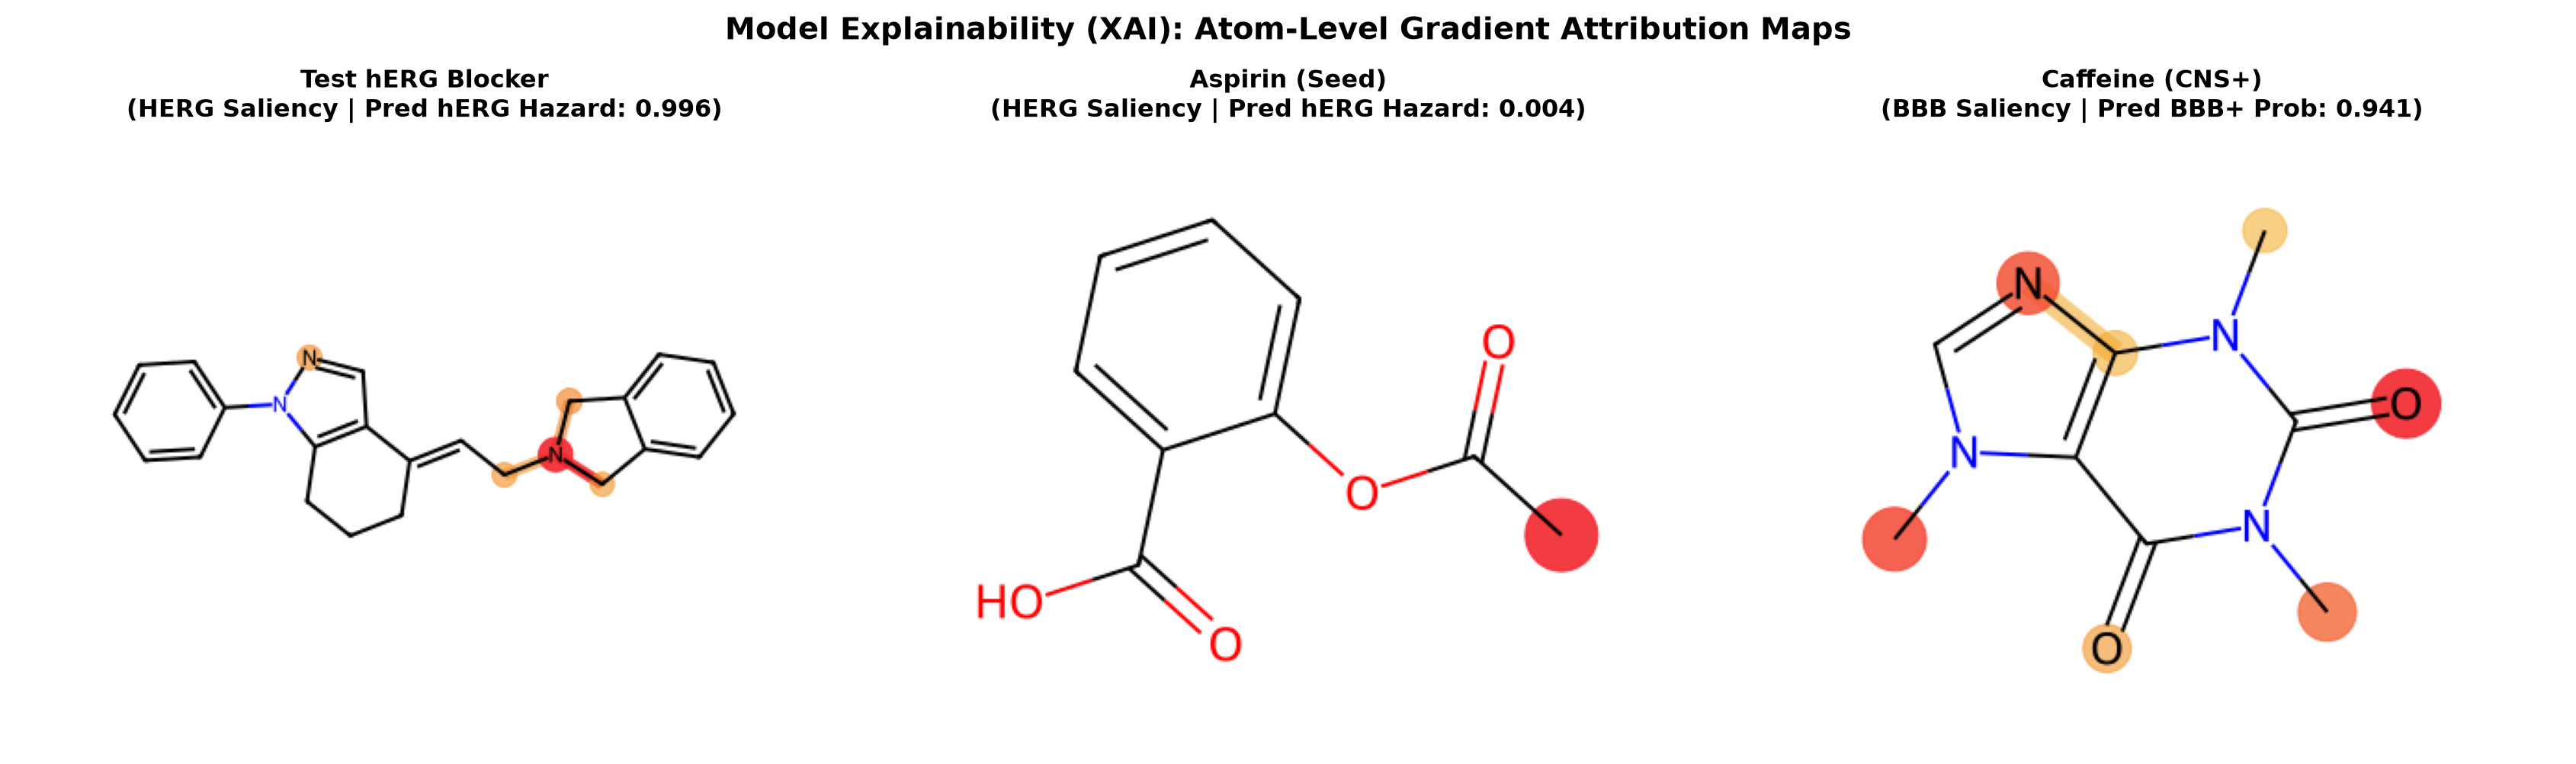
\includegraphics[width=\linewidth]{../results/figures/07_atom_saliency_xai.png}
\caption{Input $\times$ Gradient atom attribution maps highlighting the tertiary amine hERG pharmacophore on an unseen test blocker ($\text{hERG}=0.996$), safe Aspirin ($\text{hERG}=0.004$), and CNS-penetrant Caffeine ($\text{BBB}=0.941$).}
\label{fig:xai}
\end{figure}

\section{Discussion, Honest Limitations, and Future Work}
To uphold strict scientific transparency, several empirical boundaries must be noted:
\begin{enumerate}
    \item \emph{Single-Seed Evaluation:} Results reflect deterministic seed \texttt{42}; multi-seed confidence intervals remain to be quantified.
    \item \emph{Small Bioavailability Test Split:} Because \texttt{Bioavailability\_Ma} contains 636 compounds total, the scaffold-disjoint test fold contains $n=44$ labeled samples, introducing moderate ROC-AUC variance relative to hERG ($n=330$).
    \item \emph{Binary vs. Continuous Bioavailability:} The bioavailability head predicts $P(F \ge 20\%)$ scaled to $[0, 100]\%$ rather than continuous human percentage bioavailability.
    \item \emph{Calibrating Surrogate QED Against Exact Descriptors:} On Aspirin, the neural head predicts $\text{QED}=0.739$ versus exact RDKit $\text{QED}=0.550$ (despite overall test $R^2=0.7165$), motivating our inclusion of exact RDKit QED/SAScore checks alongside neural ADMET predictions during Stage~3 optimization.
    \item \emph{Static Single Conformer:} Each molecule uses a single ETKDGv3 conformer rather than Boltzmann-weighted multi-conformer ensembles or explicit-solvent molecular dynamics.
\end{enumerate}
Future work will extend this framework to multi-conformer SE(3)-equivariant encoders, additional endpoints (CYP450 inhibition and Ames mutagenicity), and generative 3D scaffold diffusion.

\section{Conclusion}
We presented an audited, zero-leakage Self-Supervised 2D+3D Hybrid GraphGPS framework for multi-objective ADMET profiling and evolutionary lead optimization. Across 5,007 standardized TDC clinical compounds evaluated strictly on unseen Bemis-Murcko scaffolds, contrastive pre-training on 5,000 ZINC250k molecules boosted Macro ROC-AUC by +3.43 pp to \textbf{0.8299}, outperforming ECFP4 Random Forests, Standard-GCN, and non-pretrained GraphGPS across every task while delivering interpretable atom-level saliency and PAINS-free Pareto-optimal analogues.

\bibliographystyle{IEEEtran}
\bibliography{references}

\end{document}
